

%%%%%%%%%%%%%%%%%%%%%%%%%%%%%%%%%%%%%%%%%%%%%%%%%%%%%%%%%%%%%%%%%%%%%%%%%%%%%%%%
%%%
%%% тема лекции
%%%

\section{Теория}

\subsection{Обработка данных}

В качестве препроцессинга данных и приведения их к удобоиспользуемому виду я предлагаю использовать стандартный подход \textbf{word embedding}. Он заключается в том, что каждому слову сопоставляется вектор в некотором многомерном векторном пространстве. Чаще всего вектор подбирают таким образом, чтобы они каким-то образом характеризовали семантическое положение слова относительно остальных.

\begin{center} 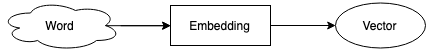
\includegraphics[width=370pt]{images/model_schema_1.png}\end{center}

Довольно известен пример такого проецирования из работы Томаша Миколова [2, 3], одного из основоположников теории world2vec.

\begin{center} 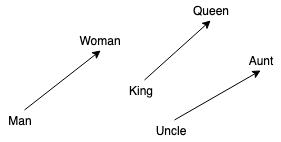
\includegraphics[width=300pt]{images/model_schema_2.png}

Можно видеть, что взаимное расположение\\ \textbf{Woman} и \textbf{Man} близко к \textbf{Queen} и \textbf{King}, \textbf{Aunt} и \textbf{Uncle}.\end{center}

В рамках этой работы мы не будем рассматривать способы проецирования слов в векторное пространство. Мы возьмем уже готовые широкоиспользуемые словари, подготовленные на основе больших корпусов текстов: \textbf{glove}, \textbf{wiki-news}, \textbf{GoogleNews}, \textbf{paragram}.

Наш \textbf{word embedding} для конкретного слова будет представлять собой конкатенацию векторов из всех этих словарей. Предполагается, что полученные таким образом векторы будут давать хорошую возможность для обучения описанной далее модели.

\subsection{Модель}

Обозначим требования к модели, которая должна получиться в результате:
\begin{itemize}
    \item Способность выделять тему, контекст и ключевые слова в предложении
    \item Обладание долговременной памятью о предыдущих предложениях
    \item Обладание кратковременной памятью о предыдущих словах при их последовательной обработки
\end{itemize}


\subsubsection{Нейронная сеть}
Рассмотрим обычную нейронную сеть. Как мы знаем, общих чертах она представляет из себя набор слоев из нейронов,  последовательно соединенных друг с другом. На вход она принимает вектор, пропускает его значения через все связи с весами, вычисленными в процессе обучения и в выходном слое выдает некоторую величину.

\begin{center} 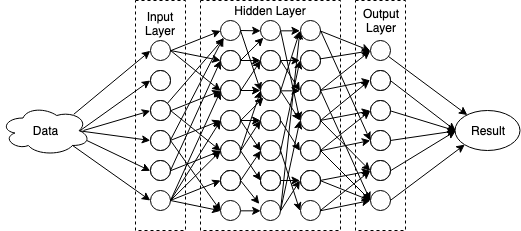
\includegraphics[width=450pt]{images/model_schema_3.png} \end{center}

Однако без доработок эта модель не запоминает свои предыдущие решения, а работает только в текущем контексте. Для исправления этого недостатка была разработана теория рекуррентных сетей.


\subsubsection{Рекуррентная сеть}

В рекуррентной сети добавляется сохранение некоторых состояний и передача их в дополнительным входным потоком при последующих запусках: 

\begin{center} 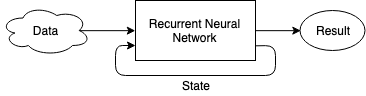
\includegraphics[width=330pt]{images/model_schema_4.png} \end{center}

Для удобства понимания можно представить эту схему как набор одинаковых сетей, каждая из которых передает состояние в предыдущую:

\begin{center} 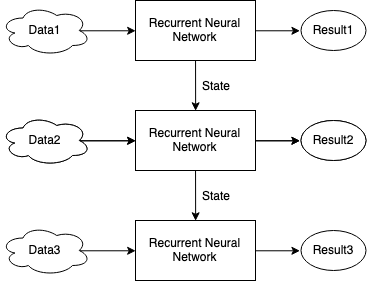
\includegraphics[width=300pt]{images/model_schema_5.png} \end{center}

Такое устройство сети в целом уже может удовлетворять основным нашим потребностям. Она умеет распознавать ключевые слова и способна последовательно обрабатывать различные синтаксические единицы, уделяя внимание контексту, образованному раннее.

Но мы пойдем дальше и будем использовать более сложноые, усовершенствованные рекуррентные сети под названием \textbf{LSTM} (от англ. \textit{Long short-term memory}).


\subsubsection{LSTM}
Усовершенствование заключается в введении механизмов управления памятью через регулирующие ее сущности, помогающие определить ценность информации для запоминания и фокусироваться только на тех вещах, которые нужны в текущий момент [1]. В литературе обычно говорят о трех таких механизмах:

\begin{itemize}
    \item \textbf{Forget gate} - механизм, определяющий подмноженство данных из долговременной памяти, которое необходимо забыть в текущем запуске.
    \item \textbf{Input gate} - механизм, определяющий подмножество данных, которое необходимо положить в долговременную память в текущем запуске.
    \item \textbf{Output gate} - механизм, определяющий подмножество данных из долговременной памяти, которое необходимо положить в кратковременную в текущем запуске.
\end{itemize}

Общепринятое название этих механизмов - \textbf{вентили}. Каждый из них реализован как сигмоида:

$$\sigma(x) = \frac{1}{1 + e^{-x}}$$

Используя внутреннюю память $c_t$, на каждом шаге работы сети вычисляется не только скрытое состояние $h_t$, но и вектор памяти $c_t$ [1]. Более подробные формулы вычисления вентилей:

$$f_t = \sigma(W_f x_t + U_f h_{t - 1} + b_f), ~i_t = \sigma(W_i x_t + U_t h_{t - 1} + b_i), ~ o_t = \sigma (W_o x_t + U_o h_{t - 1} + b_o)$$

Такой подход позволяет не зависеть от того, как давно была полученна важная информация. Если сеть видит, что она важна, она не будет забывать ее.

\subsubsection{BiLSTM}

Как можно понять, LSTM является итеративным алгоритмом, который проходит по словам в последовательном порядке. В качестве некоторого улучшения многие исследователи используют \textbf{бинаправленность} - добавляют к естественному порядку инвертированный. То есть, сеть проходит сначала слева направо, а потом справа налево. [5]

На практике такое решение дает некотороый прирост к качеству предсказаний.

\subsubsection{GRU}
Еще одна независимая от LSTM архитектура рекуррентных сетей называется \textbf{GRU} (от англ. \textit{Gated Recurrent Units}). Она была представлена в 2014 и отличается тем, что не содержит \textbf{Output gate}, а, значит, содержит на четверть меньше данных для обработки. [6]

В рамках этой работы мы только упомянем эту архитектуру и не будем глубоко погружаться в устройство ее работы.


\subsection{Постпроцессинг}

Выходом нейронной сети является некоторое вещественное число, которое с помощью операции \textbf{softmax} проецируется в отрезок [0, 1]. После этого наша задача найти такой порог определения в классы, при котором используемая в задаче F - мера покажет наилучший результат.


\pagebreak
